\documentclass{jfm}

\usepackage{xcolor}
\usepackage{array}
\usepackage{longtable}

\usepackage{graphicx,color}
% \usepackage[section]{placeins}
\usepackage{float}
\usepackage{graphicx,subfigure}
\usepackage{epstopdf, epsfig}
\usepackage{amstext}
\usepackage{amsmath}
\usepackage{todonotes}
\usepackage{hyperref}
\usepackage{verbatim}
\usepackage{bm}
\usepackage{diagbox}
\usepackage{forloop}

\newtheorem{theorem}{Theorem}
\newtheorem{defn}{Definition}
\newtheorem{lemma}{Lemma}
\newtheorem{corollary}{Corollary}
\newtheorem{prop}{Proposition}
\newtheorem{assume}{Assumption}
\newtheorem{notation}{Notation}
\DeclareMathOperator*{\argmin}{arg\,min}

\newcommand\nc{\newcommand}
\nc\qu{\quad}
\nc\tends{\rightarrow}
\nc\dint{\int\!\int}
\newcommand{\vect}[1]{\mbox{\boldmath $#1$}}
\nc{\degree}{\mbox{\footnotesize{o}}}

\newcommand{\bes} {\begin{eqnarray*}}
\newcommand{\ees} {\end{eqnarray*}}
\newcommand{\dd} \partial

\newcommand{\non} \nonumber
\newcommand{\ie}{{\it i.e.}\ }
%\newcommand{\eg}{{\it e.g.}\ }
%\newcommand{\etal}{{\it et al.} \ }
\newcommand{\ru}{R_{\rm u}}
\newcommand{\rb}{R_{\rm b}}
\newcommand{\qup}{Q_{\rm u,pore}}
\newcommand{\qbp}{Q_{\rm b,pore}}

\newcommand{\ra}{\rightarrow}

\nc\cA{{\cal{A}}}
\nc\cB{{\cal{B}}}
\nc\cZ{{\cal{Z}}}
\nc\cX{{\cal{X}}}
\nc\cS{{\cal{S}}}
\nc\cR{{\cal{R}}}
\nc\cW{{\cal W}}
\nc\cU{{\cal U}}
\nc\cP{{\cal P}}
\nc\cF{{\cal{F}}}
\nc\cG{{\cal{G}}}
\nc\bz{\bar{z}}
\nc\bZ{\bar{Z}}
\nc\baz{\bar{\zeta}}
\nc\bw{\bar{w}}
\nc\bW{\bar{W}}
\nc\bX{\bar{X}}
\nc\bet{\bar{\eta}}
\nc\bp{\bar{\phi}}
\nc\bP{\bar{\Phi}}
\nc\bc{\bar{\chi}}
\nc\baf{\bar{f}}
\nc\baF{\bar{F}}
\nc\ov{\overline}
\nc\oW{\ov{W}}

\nc\hA{\hat{A}}
\nc\hB{\hat{B}}
\nc\ho{\hat{O}}
\nc\hG{\hat{\Gamma}}
\nc\hS{\hat{S}}
\nc\hO{\hat{\Omega}}
\nc\bO{\ov{\Omega}}
\nc\gham{\hat{\gamma}}
\nc\gcam{\check{\gamma}}
\nc\z{\zeta}
\nc\s{\sigma}
\nc\ep{\epsilon}
\nc\up{\upsilon}
\nc\lam{\lambda}
\nc\sig{\sigma}
\nc\om{\omega}
\nc\kap{\kappa}
\nc\gam{\gamma}
\nc\pa{\partial}
\nc\dom{\pa\Omega}
\nc\domt{\pa\tilde{\Omega}}
\nc\doh{\pa\hat{\Omega}}
\nc\pad[2]{\frac{\pa #1}{\pa #2}}
\nc\padd[2]{\frac{\pa^2 #1}{\pa {#2}^2}}
\nc\pard[3]{\frac{\pa^2 #1}{\pa {#2}\pa {#3}}}
\nc\nd[2]{\frac{d #1}{d #2}}
\nc\ndd[2]{\frac{d^2 #1}{d {#2}^2}}
\nc\ds{\displaystyle}
\nc\del{\nabla}
\nc\lap{\nabla^2}
\nc\ud{|\z|\leq 1}

\nc\capil{\mbox{Ca}}

\nc\pt{\tilde{a}}
\nc\ft{\tilde{f}}
\nc\vt{\tilde{v}}
\nc\wt{\tilde{w}}
\nc\nt{\tilde{\nu}}
\nc\xit{\tilde{\xi}}
\nc\xt{\tilde{x}}
\nc\etat{\tilde{\eta}}
\nc\nht{\tilde{\hat{\eta}}}
\nc\Taut{T}
\nc\zt{\tilde{\z}}
\nc\nut{\tilde{\nu}}

\nc\At{\tilde{\cA}}
\nc\qt{\tilde{B}}
\nc\Ct{\tilde{C}}
\nc\dt{\tilde{D}}
\nc\Dt{\tilde{\cU}}
\nc\Et{\tilde{L}}
\nc\Ft{\tilde{F}}
\nc\Ht{\tilde{H}}
\nc\Kt{\tilde{K}}
\nc\Lt{\tilde{K}}
\nc\Mt{\tilde{M}}
\nc\Nt{\tilde{N}}
\nc\Pt{\tilde{\Phi}}
\nc\Qt{\tilde{Q}}
\nc\Rt{\tilde{R}}
\nc\St{\tilde{\cS}}
\nc\Wt{\tilde{W}}
\nc\cWt{\tilde{\cW}}
\nc\Xt{\tilde{X}}

\nc\vs{\varsigma}
\nc\vp{\varpi}
\nc\ve{\varepsilon}
\nc\vepa{\ve_{\parallel}}
\nc\vepe{\ve_{\perp}}

%\bibliographystyle{elsarticle-num}


%\nc\captionsize{\footnotesize}

\newcommand{\pejman}[1]{\todo[inline,color=green!40]{Pejman: #1}}
\newcommand{\daniel}[1]{\todo[inline,color=yellow!40]{Daniel: #1}}
\newcommand{\michael}[1]{\todo[inline,color=red!40]{Michael: #1}}
\newcommand{\charles}[1]{\todo[inline,color=blue!40]{Charles: #1}}

\newcolumntype{A}[2]{%
    >{\minipage{\dimexpr#1\linewidth-2\tabcolsep-#2\arrayrulewidth\relax}\vspace\tabcolsep}%
    c<{\vspace\tabcolsep\endminipage}}

\newenvironment{lapsetable}[2]{ % n_cols, wid
    \tabular{
        |c|c|
        *{#1}{>{\centering}A{#2}{1.5}|}
    }
    \ignorespaces
    }{
    \tabularnewline\hline
    \endtabular\ignorespacesafterend
}
\newenvironment{shortlapsetable}[2]{ % n_cols, wid
    \tabular{
        |c|
        *{#1}{>{\centering}A{#2}{1.5}|}
    }
    \ignorespaces
    }{
    \tabularnewline\hline
    \endtabular\ignorespacesafterend
}
\newenvironment{sslapsetable}[2]{ % n_cols, wid
    \tabular{
        |
        *{#1}{>{\centering}A{#2}{1.5}|}
    }
    \ignorespaces
    }{
    \tabularnewline\hline
    \endtabular\ignorespacesafterend
}

\newcounter{lapse_iter}
\newcommand{\lapse}[9]{ % name, dt, N, dt_display, n_cols, *crop
    \tabularnewline\hline
    #3 & #4
    \forloop{lapse_iter}{1}{\not{\value{lapse_iter} > #5}}{
        &
        \includegraphics[width=\textwidth, trim={#6cm #7cm #8cm #9cm}, clip]{tableFigs/#1/output_#2_#3/\arabic{lapse_iter}.png}
    }
}
\newcommand{\lapseShort}[6]{ % name, n_cols, width, *crop
    \forloop{lapse_iter}{1}{\not{\value{lapse_iter} > #2}}{
        &
        \includegraphics[width=\textwidth, trim={#3cm #4cm #5cm #6cm}, clip]{tableFigs/#1/\arabic{lapse_iter}.png}
    }
}
\newcommand{\scinote}[2]{${#1}\times10^{#2}$}

\shorttitle{Droplets on a wall}
\shortauthor{M. Li et al.}

\title{Droplets on a Wall: Moving Contact Lines with the Immersed Boundary Method}
\author{Michael Y. Li$^{1*}$, Daniel Chin$^{2*}$, Charles Puelz\aff{3}, Pejman Sanaei\aff{4}\corresp{\email{psanaei@nyit.edu}}}
\affiliation{
    \aff{1}
    Courant Institute of Mathematical Sciences, New York University,\\ New York, NY 10012-1110, USA\\
    \aff{2}
    New York University Shanghai,\\ Shanghai, 200120, China\\
    \aff{3}
    Department of Pediatrics, Section of Cardiology, Texas Children's Hospital and Baylor College of Medicine, Houston, TX 77030-????, USA\\
    \aff{4}
    Department of Mathematics, New York Institute of Technology,\\ New York, NY 10023-7692, USA\\
    $^{*}$M. Y. Liu and D. Chin contributed equally to this work.
}

\begin{document}
\maketitle
\begin{abstract}
In this work, we use the Immersed Boundary (IB) method to simulate the movement of 2D liquid droplets hanging on a vertical wall. The simulation requires a moving contact line (MCL) model and a surface tension model that work well with IB. We propose an MCL model that enforces Navier slip on penalty-simulated immersed boundaries. The static and dynamic contact line angle are endogenous instead of prescribed. We use a liquid-gas interface model that is capable of simulating both surface tension force and unbalanced Young's force with one general equation, which does not involve estimating local curvature. We also employ a step-wise re-sampling technique to ensure the uniform distribution of the Lagrangian markers that represent the liquid-gas interface and a step-wise interface splicing method to implement droplet coalescence and separation. 
\end{abstract}

\section{Introduction}
Problems involving the two-way coupling between a fluid and some evolving immersed boundaries are often difficult to model analytically. The Immersed Boundary (IB) method is a numerical method that solves the two-way coupling problem with an elegant assumption that the immersed boundaries are massless \cite{peskin1972flow}. IB represents the fluid with a Eulerian velocity field and the immersed boundaries with arrays of linked Lagrangian markers. The fluid advects the markers and the markers exert forces onto the fluid. 

The massless-boundary assumption is suitable for describing thin elastic membranes common to biological contexts, for example, the interaction between blood flow and heart valves \cite{peskin1972flow}. Similarly, the massless-boundaries assumption is appropriate for liquid-gas interfaces. Thus, with a surface tension model, IB is capable of modelling multi-phase fluid flow \cite{surface_tension_review, surface_tension_IB_estimates_curvature, multi_phase_2018, assessment_VOF_vs_IB}. The next challenge is the moving contact line (MCL) problem that emerges when a solid boundary meets with a liquid-gas interface. \cite{MCL_IBM_surfactant} proposes an MCL model that simulates Navier slip with IB, but it is limited to \textit{fixed} solid boundaries. In this work, we simulate Navier slip between a moving liquid-gas interface and an \textit{evolving} immersed solid boundary. Two types of immersed boundaries (liquid-gas interface, solid surface) coexist and are governed by the same IB numerical method. The Navier slip condition is informed by a recent (2018) molecular dynamics (MD) simulation \cite{MD_2018_its_the_bonds}. The resulting simulation scheme, unlike related works that either prescribe the contact angle \cite{curved_solid_DI_IB, muradoglu2010front} or specify marker velocity \cite{manservisi2009variational}, is capable of reaching the \textit{static} contact angle and the \textit{dynamic} contact angle in an endogenous way. 

In addition to the MCL model, we propose a surface tension model with IB. Using IB to simulate surface tension is often classified as a front-tracking method. Most front-tracking methods, including many IB variants, compute the magnitude of surface tension by estimating the local curvature of the interface from about three to six markers \cite{surface_tension_IB_estimates_curvature, multi_phase_2018}, which is susceptible to errors and instability issues if not specifically combated \cite{assessment_VOF_vs_IB}. \cite{surface_tension_still_tangent_applied_to_segment} computes the surface tension using tangent vector subtraction in every Eulerian cell, thus nullifying the need to estimate curvature. \cite{eulerian_tension_lagrangian_advection} uses tangent vector subtraction for every link between adjacent Lagrangian markers, exploiting the advantage of IB. Our method uses tangent vector summation for every Lagrangian marker (instead of every link). The subtle shift in perspective brings an interesting side effect that the unbalanced Young's force at the three-phase intersection is readily computed by the two markers at both ends of a liquid-gas interface. 

We also employ a step-wise re-sampling technique to ensure the uniform distribution of Lagrangian markers in the liquid-gas interface. Finally, we employ a step-wise interface splicing method to implement droplet coalescence and separation. 

We use our methods to simulate 2D droplets moving on a vertical wall. This scenario is based on a real-life case where a vertical catalyst scaffold removes pollutants such as sulfur dioxide (SO2) from industrial exhaust before release into the atmosphere \cite{MPIreport2018}, which is of considerable environmental interest. We measure the spatial and temporal convergence of our methods. We compare simulation results at equilibrium against the analytical solution. We benchmark our methods with several standard test cases. 

\section{Numerical methods} \label{sec:numerical}
We next implement computational fluid dynamics simulations of the flow around droplets using the Immersed Boundary (IB) method in order to extract torque-orientation profiles. The IB method has proven to be a versatile method for such fluid-structure interaction problems since its development almost forty years ago \citep{peskin1972flow,mcqueen1997shared,arthurs1998modeling,lai2000immersed,griffith2009simulating,balboa2011staggered,devendran2012immersed,ibamradaptive}. The method describes the solid structure with Lagrangian or co-moving coordinates and the fluid with Eulerian or `lab frame' coordinates, where the forces of interaction between the two are communicated locally in a manner consistent with Newton's laws. For the rigid and fixed bodies considered here, we adopt the Penalty Immersed Boundary Method \citep{kim2016penalty}, which introduces a third set of \textit{tether points} that are absolutely fixed in space and represent the desired shape and location of the solid boundary. The boundary points are connected to the tether points via springs, and it is only the boundary points that interact with the fluid. Stiff springs approximate a rigid boundary, at the cost of numerical stiffness but with the benefit of ease of implementation. In practice, accurate results can be achieved with appropriate choices of spring constant, spatial discretization, time-stepping, and other numerical parameters \citep{kim2016penalty}. 

The continuum form of the coupled fluid-solid dynamical equations are:
\begin{align}
\rho(\cfrac{\partial\bm{u}}{\partial t}+\bm{u}\cdot\nabla\bm{u}) & =-\nabla p+\mu\Delta\bm{u}+\bm{f},\quad
\nabla\cdot\bm{u}=0, \label{1}\\
\bm{f}(\bm{x},t) & =\int\bm{F}(s,t)\delta(\bm{x}-\bm{X}(s,t))ds, \label{2}\\
\cfrac{\partial\bm{X}}{\partial t}(s,t)=\bm{U}(\bm{X}(s,t),t) & =\int\bm{u}(\bm{x},t)\delta(\bm{x}-\bm{X}(s,t))d\bm{x}, \label{3}\\
\bm{F}(s,t) & =-k(\bm{X}(s,t)-\bm{Z}(s,t)). \label{4}
\end{align}
Here $\rho$ and $\mu$ are the density and viscosity of the fluid and $k$ is a spring constant; $\boldsymbol{x}$ and $\boldsymbol{X}$ are the Eulerian fluid coordinate and the Lagrangian boundary coordinate; $\boldsymbol{u}(\boldsymbol{x},t)$ and $\boldsymbol{U}(\boldsymbol{X}(s,t),t)$ represent the fluid and solid velocities; $\boldsymbol{f}$ and $\boldsymbol{F}$ are the Eulerian and the Lagrangian force densities; and $\delta$ is a 2D delta function. Equation (\ref{1}) is the Navier-Stokes equation describing incompressible flow of a viscous fluid. Equation (\ref{2}) describes how force is imparted from the boundary to the fluid. Equation (\ref{3}) ensures the boundary moves with the local flow field, which invokes the no-slip boundary condition. Equation (\ref{4}) describes the tether-point construction and the associated spring force on the boundary. Here, $\boldsymbol{Z}$ and $\boldsymbol{X}$ are the locations of tether and solid boundary points, respectively.

\subsection{Wall as an Immersed Boundary} \label{subsec:wall}
The main case that motivates our study is simulating liquid droplets moving on a solid, vertical wall. We simulate the wall as an immersed boundary. In this specific case, because the wall is static, It is arguably easier to treat the wall as a boundary condition. However, we want our MCL method to generalize to non-static solid surfaces (for example, \ref{subsubsec:letters}), so we treat the wall as an immersed boundary anyway. Each Lagrangian marker of the wall is tethered to its starting location, thus ensuring no flux and no slip. 

\subsection{Surface Tension}
We use the integral formulation to model surface tension \cite{surface_tension_review} so each interface marker is pulled by its two neighbors at constant magnitude. In contrast with \cite{surface_tension_still_tangent_applied_to_segment}, our method is entirely in the Lagrangian domain and does not estimate a tangent vector. 

To further justify our approach, we underline that the 2D tension energy is proportional to the interface length. If we view that as the sum of all line segments connecting neighboring markers, then an attractive force with constant magnitude is precisely the gradient of the length of one line segment. Apply that to all line segments and each interface marker will be pulled by its two neighbors at constant magnitude. Note that the total force on any one marker is always normal to the interface. 

A consequence of this implementation is that the unbalanced Young’s force at the three-phase contact points are correctly simulated as a side effect. At the three-phase contact point, there is one interface marker that only has one neighbor. The total force on this marker becomes tangent, instead of normal, to the interface. The horizontal component of this force is balanced by the no-flux force provided by the wall. Notice that the sum of the tension force on all markers is exactly the sum of unbalanced Young’s force on the two markers, just inverted in direction. 
\daniel{image}

\subsection{Moving Contact Line and Navier Slip}
The moving contact line (MCL) problem refers to the apparent contradiction that contact lines can move on a no-slip wall. The mechanism of MCL and how to simulate it had been largely a mystery until 1980 \cite{1979_MCL_confusion}. Many numerical methods have tried to model MCL \cite{2014_MCL_review, curved_solid_DI_IB}. A recent study \cite{its_the_bonds_original} finds that it is the hydrogen bonds that facilitate the no-slip behavior of water on hydrophilic surfaces, which are orders of magnitudes stronger compared to internal viscosity, which justifies the validity of the no-slip assumption in non-MCL scenarios. In an MCL, the hydrogen bonds do break, allowing slip. The energy dissipation is quantified by a molecular dynamics (MD) simulation \cite{MD_2018_its_the_bonds}. Therefore, it is proper to treat the wall a Navier-slip where there is an MCL. For example in \cite{MCL_IBM_surfactant}, MCL is simulated with IB by giving Navier slip boundary condition to the fluid solver. However, if the geometry of the solid boundary evolves with time, imposing it onto the fluid will be difficult. This section proposes a method to implement Navier slip on an immersed boundary. 

First we include a static friction component in the friction scheme: 
\begin{equation}
    f=\min\{|F_Y|,f_\text{limit}\}
    \cdot
    \left(
    -\frac{F_Y}{|F_Y|}
    \right)
\end{equation}
\begin{equation}
    f_\text{limit}=
    f_{\text{min}}+\mu(\theta)
    \cdot
    |\vec{u}\cdot\hat{j}|
\end{equation}
where $f$ is the resulting wall friction, $f_\text{limit}$ the critical wall friction, $F_Y$ is the local unbalanced Young's force, $f_{\text{min}}$ is the minimum friction force (an exogenous parameter allows partial no slip), $\theta$ is the contact angle, $\mu$ is a function that gives a friction coefficient without unit, $\vec{u}$ is the local fluid velocity, and $\hat{j}$ is the vertical unit vector.

Function $\mu(\theta)$ computes the friction coefficient given the contact angle. Our implementation of $\mu(\theta)$ is based on a regression of measured results yielded from \cite{MD_2018_its_the_bonds}. 
\daniel{psuedo code}

We believe more accurate results can be obtained from fine-tuning $\mu(\theta)$ based on MD studies such as \cite{MD_navier}. 

The resulting macroscopic behaviors are analogous to static friction and sliding friction. When the contact angle is large enough such that $|F_Y|<F_\text{limit}$, the contact point is non-slip, hence $f=-F_Y$, which is identical to the no-slip condition. 

Here is how we integrate this friction into IB. Subsection \ref{subsec:wall} describes the penalty method we use to simulate a no-slip wall. To simulate a Navier-slip wall, we use what we call the \textit{incur-redeem-dismiss} penalty method. In this view, the no-slip penalty method would be an \textit{incur-redeem} penalty method. 

In the no-slip penalty method, as a marker moves away from its initial location, penalty is \textit{incurred}. A penalty force brings it back. The penalty will never be fully \textit{redeemed} until the marker returns to its correct location. This guarantees no flux and no slip. 

Now we introduce another way penalty can decrease: \textit{dismissal}. No fluid flow is involved. Penalty is instantly decreased within a timestep by displacing the marker. The amount of penalty dismissed, multiplied by friction force, gives the work done (or in other words, heat dissipation). 
\daniel{image}

\daniel{in "results": how slip only happens near contact line and smaller droplets still no slip}

\subsection{Frame-wise Interface Re-sampling}
Surface tension is always normal to the interface. The absence of a tangential component allows the fluid flow to easily disrupt the distribution of interface markers. To equi-distribute the markers, \cite{lai2008immersed} uses grid redistribution, while \cite{hou1994removing, MCL_IBM_surfactant} apply artificial tangential velocity. Our method is similar to grid distribution, adding markers to wide gaps and removing markers from tight spaces every timestep. 
[image comparison in compareresample.mp4]

This re-sampling technique, however, is very difficult to implement in 3D where the point array becomes a surface mesh.  

\subsection{Interface Splicing}
There are six conceivable scenarios where the interface needs to be spliced: Two droplets merging, one droplet splitting into two, droplet attaching onto the wall, droplet detaching from the wall, droplet splitting at the wall, and droplets merging at the wall. 

[image]
Image caption: Here there are three pairs of reversed processes. And three pairs of scenarios whose implementations are exactly the same. They are locally indistinguishable, since we don't care about liquid and gas switching sides. 

To implement splicing, we store the interface markers in circular double linked lists. The linking direction preserves the polarity information: if one follows the links in the positive direction, the liquid will always be on the right. When the distance between two interfaces is smaller than a threshold and the two interfaces are approaching, splice them. In our simulations, we have two different thresholds, one for interface-interface events ($h$), and the other for interface-wall events ($2.3h$), where $h$ is the meshwidth (i.e. length of one Eulerian grid cell). 

The following two timesteps then become a no-splice window. This rule makes splicing events more atomic so that there will not be multiple splicing events competing to accomplish the same macroscopic effect. 

Computation-wise, a naive algorithm would check every pair of markers at every timestep. This is $O(N^2)$. We check every pair of markers only once in a while and mark anything close together as suspects. At each timestep we only check the suspect markers. This greatly enhances simulation efficiency. The time interval between global checks is dynamic, computed by dividing the minimum interface distance with the maximum marker velocity, multiplied by $1/2$ and some safeguarding constant. More specifically, our implementation involves maintaining a moving window of past extreme velocities and taking the 40\% percentile. 

\subsection{Surface Resampling \& Splicing}\label{sec:results}
Surface tension is always normal to the interface. The absence of a tangential component allows the fluid flow to easily disrupt the distribution of interface markers. To equi-distribute the markers, \cite{lai2008immersed} uses grid redistribution, while \cite{hou1994removing, MCL_IBM_surfactant} apply artificial tangential velocity. Our method is similar to grid distribution, adding markers to wide gaps and removing markers from tight spaces every timestep. 
[image comparison in compareresample.mp4]

This re-sampling technique, however, is very difficult to implement in 3D where the point array becomes a surface mesh.

There are six conceivable scenarios where the interface needs to be spliced: Two droplets merging, one droplet splitting into two, droplet attaching onto the wall, droplet detaching from the wall, droplet splitting at the wall, and droplets merging at the wall. 

[image]
Image caption: Here there are three pairs of reversed processes. And three pairs of scenarios whose implementations are exactly the same. They are locally indistinguishable, since we don't care about liquid and gas switching sides. 

To implement splicing, we store the interface markers in circular double linked lists. The linking direction preserves the polarity information: if one follows the links in the positive direction, the liquid will always be on the right. When the distance between two interfaces is smaller than a threshold and the two interfaces are approaching, splice them. In our simulations, we have two different thresholds, one for interface-interface events ($h$), and the other for interface-wall events ($2.3h$), where $h$ is the meshwidth (i.e. length of one Eulerian grid cell). 

The following two timesteps then become a no-splice window. This rule makes splicing events more atomic so that there will not be multiple splicing events competing to accomplish the same macroscopic effect. 

Computation-wise, a naive algorithm would check every pair of markers at every timestep. This is $O(N^2)$. We check every pair of markers only once in a while and mark anything close together as suspects. At each timestep we only check the suspect markers. This greatly enhances simulation efficiency. The time interval between global checks is dynamic, computed by dividing the minimum interface distance with the maximum marker velocity, multiplied by $1/2$ and some safeguarding constant. More specifically, our implementation involves maintaining a moving window of past extreme velocities and taking the 40\% percentile. 

\subsection{Variable Density}
The liquid phase and and gas phase have different density. The variable density technique proposed in \cite{IBM_variable_density} uses another set of Lagrangian markers to represent density difference. The fluid solver is still global and is not aware of the density difference. The density difference markers are tethered to their Newtonian and massive counterpart with the penalty method, thus correctly simulating gravitational and inertial differences.

In our simulation we employ their variable density method with some modifications. Instead of their five-step update method, we use a coarser, midpoint method. We also set the allowed distance (between a marker and its Newtonian counterpart) to be one tenth the meshwidth ($h/10$). 

%\section{Scaling \& nondimensionalization\label{sec:scaling}}
\subsection{Dynamic Slipping}\label{sec:results}
We implement our numerical method for tension force. Each interface marker is pulled by its two neighboring markers at a constant magnitude. In our 2D case, the tension energy is proportional to the interface length, which can be described as the sum of all line segments. An attractive force with constant magnitude is the gradient of the length of one line segment. The total force on a marker is always normal to the interface. Using this method, we can simulate the unbalanced Young's force at a contact point. At the wall, there is a marker that has only one neighboring marker. In this case, the total force on this marker becomes tangent to the interface. Its horizontal component is balanced by the non-flux force provided by the wall, and its vertical component is the Young's force. The sum of the tension force on all markers is exactly the sum of Young's force on the two markers, with opposite directions. We can view them as pair of action-reaction forces.

The dynamical slipping scheme is inspired by a study, which has partially revealed the microscopic model for hydrophilic surface interaction (Johansson \& Hess 2018;Ref). The scheme explains how we can simulate friction with slip wall. We focus on 2D from here on:
\begin{equation}
    f=\min\{|F_Y|,f_\text{limit}\}\cdot\left(-\frac{F_Y}{|F_Y|}\right)
\end{equation}
\begin{equation}
    f_\text{limit}=f_{\min}+\mu(\theta)\cdot|\boldsymbol{u}\cdot\boldsymbol{j}|
\end{equation}
where $f$ is the wall friction, $f_\text{limit}$ the critical wall friction,$F_Y$ is the local Young's force, $f_{\min}$ is the minimum friction force, $\theta$ is the contact angle, $\mu$ is the friction coefficient, $\boldsymbol{u}$ is the local fluid velocity, and $\boldsymbol{j}$ is the vertical unit vector.

The results of $\mu(\theta)$ are computed based on a regression of results (Johansson \& Hess 2018). (Add figure here)

When the contact angle is large enough such that $|F_Y|<F_\text{limit}$, the contact point is non-slip, hence $f=-F_Y$, which is identical to the non-slip case.

\subsection{Non-Slip Conditions}
At the contact point, Young's force is tangential to the wall, and the tension force is normal to the interface. Tension force can be neglected compared to Young's force in this case.

We can view the non-slip boundary conditions as a friction force, provided by the wall and exerted onto the fluid. Non-slip means the friction is a reactive force, balancing the sum of active forces at the point in the vertical direction. Nonslip friction balances Young's force at the wall. Friction is easy to solve when the active forces are readily computed in a numerical scheme.

Note that friction modeled here is similar to the viscous force. The viscous force is the friction between neighboring layers of the fluid, and wall friction is the friction between the wall and the first layer of the fluid.

\subsection{Variable Density}
The liquid phase and and gas phase have different density. The variable density technique proposed in \cite{IBM_variable_density} uses another set of Lagrangian markers to represent density difference. The fluid solver is still global and is not aware of the density difference. The density difference markers are tethered to their Newtonian and massive counterpart with the penalty method, thus correctly simulating gravitational and inertial differences.

In our simulation we employ their variable density method with some modifications. Instead of their five-step update method, we use a coarser, midpoint method. We also set the allowed distance (between a marker and its Newtonian counterpart) to be one tenth the meshwidth ($h/10$). 

\section {Test Cases and Results}
\subsection {Convergence Tests}
    \subsubsection {Test 1: Droplet Sliding}
        \longtable{
            A{.13}{1.5}|
            *{3}{>{\centering}A{.25}{1.5}}
        }\ignorespaces
            \diagbox[width=4.8em]{dt}{N}
            &
            96
            &
            128
            &
            192
        \tabularnewline\hline
            \scinote{5}{-5}
            &
            \includegraphics[width=30mm, trim={4.7cm 1.7cm 4cm 1.2cm}, clip]{tableFigs/slide_terminal/{output_0.000050_96}.png} 
            &
            \includegraphics[width=30mm, trim={4.7cm 1.7cm 4cm 1.2cm}, clip]{tableFigs/slide_terminal/{output_0.000050_128}.png} 
            &
            \includegraphics[width=30mm, trim={4.7cm 1.7cm 4cm 1.2cm}, clip]{tableFigs/slide_terminal/{output_0.000050_192}.png} 
        \tabularnewline
            \scinote{2}{-5}
            &
            \includegraphics[width=30mm, trim={4.7cm 1.7cm 4cm 1.2cm}, clip]{tableFigs/slide_terminal/{output_0.000020_96}.png} 
            &
            \includegraphics[width=30mm, trim={4.7cm 1.7cm 4cm 1.2cm}, clip]{tableFigs/slide_terminal/{output_0.000020_128}.png} 
            &
            \includegraphics[width=30mm, trim={4.7cm 1.7cm 4cm 1.2cm}, clip]{tableFigs/slide_terminal/{output_0.000020_192}.png} 
        \tabularnewline
        \endlongtable\ignorespacesafterend
    \subsubsection {Test 2: Coalescence of Two Droplets}
        \begin{center}
            \begin{lapsetable}{6}{.08}
                N & dt & t=0.01&0.02&0.03&0.04&0.05&0.06
                \lapse{merge2}{0.000500}{64} {\scinote{5}{-4}}{6}{5.5}{4}{4.8}{1.5}
                \lapse{merge2}{0.000200}{96} {\scinote{2}{-4}}{6}{5.5}{4}{4.8}{1.5}
                \lapse{merge2}{0.000100}{128}{\scinote{1}{-4}}{6}{5.5}{4}{4.8}{1.5}
            \end{lapsetable}
        \end{center}
        Text talks about this result
    \subsubsection {Test 3: Coalescence of Six Droplets}
        \begin{center}
            \begin{lapsetable}{6}{.13}
                N & dt & t=0.01&0.02&0.03&0.04&0.05&0.06
                \lapse{merge6}{0.000200}{96} {\scinote{2}{-4}}{6}{3.4}{3.8}{2.3}{1.5}
                \lapse{merge6}{0.000100}{128}{\scinote{1}{-4}}{6}{3.4}{3.8}{2.3}{1.5}
                \lapse{merge6}{0.000050}{192}{\scinote{5}{-5}}{6}{3.4}{3.8}{2.3}{1.5}
            \end{lapsetable}
        \end{center}
        Text talks about this result
    \subsubsection {Test 4: Letters "IB" Fall into Elastic Pouch}
        \label{subsubsec:letters}
        \begin{center}
            \begin{lapsetable}{7}{.12}
                N & dt & t=0&0.03&0.06&0.09&0.12&0.15&0.24
                \lapse{letters}{0.0005}{96} {\scinote{5}{-4}}{7}{6}{4}{5}{5}
                \lapse{letters}{0.0003}{128}{\scinote{3}{-4}}{7}{6}{4}{5}{5}
            \end{lapsetable}
        \end{center}
\subsection {Droplets on a Wall}
    \subsubsection {Case Description}
        In our case setup "droplet on a wall", the problem domain is $1cm$ by $1cm$. The top and bottom boundary condition is periodic and the left and right boundary condition is symmetric. The flow is incompressible. Liquid density is $1 g/cm^2$. Gas density is $0.1 g/cm^2$. Viscosity of both liquid and gas is $.01 g/s$. Surface tension coefficient is $50 N\times10^-5$. Gravity is $980 cm/s^2$. 
        
        There is a vertical wall at $x=0$. Its minimum static friction $f_\text{min}=25 N$. There is an upward vertical gas flow of $30 cm/s$, prescribed onto the velocity field at $y=0$. The prescribed velocity diminishes as $x$ approaches $0$ in the shape of $tanh$. 
        
        We use a global NS solver based on harmonics in the velocity field. The Fast Fourier Transform is used to accelerate the computation. 
        
    \subsubsection {Study 1: Hydro-static Equilibrium}
        We analytically solve the interface shape at hydro-static equilibrium of a droplet hanging on a vertical wall. The result shows a linear relation between the 2D curvature and the altitude $y$. We run several simulations and compare their equilibrium state against the theoretical results in Figure \ref{fig:h-curvature}. 

        The shape of the hanging droplet is determined by the following equations:\\
        \begin{center}
        $\vec{g}=g\cdot\hat{j}$\\
        $\nabla{p}=\rho\cdot{g}$\\
        $\frac{\mathrm{d}p}{\mathrm{d}y}=-\rho\cdot{g}$\\
        $p=-\rho\cdot{g}\cdot{y}+p_{\text{const.}}$
        \end{center}
        At the interface, we define the surface tension as:\\
        \begin{equation}
        p=p_{a}+\sigma\cdot{x(s)}
        \label{eqn:pressure}
        \end{equation}
        where $p_{a}$ is the air pressure, and $x(s)$ is the surface curvature. By parametrization of the surface, we get:\\
        \begin{center}
        $r(s)=x(s)\cdot\hat{i}+y(s)\cdot\hat{j}$\\
        $\hat{t}=\frac{\mathrm{d}r}{\mathrm{d}s}=x(s)'\cdot\hat{i}+y(s)'\cdot\hat{j}$
        \end{center}
        We normalize the derivative by writing $1=\left(\frac{\mathrm{d}x}{\mathrm{d}s}\right)^2+\left(\frac{\mathrm{d}y}{\mathrm{d}s}\right)^2$. We get $\left|\frac{\mathrm{d}x}{\mathrm{d}s}\right|=\sqrt{(x')^2+(y')^2}=1$\\
        We define the normal vector as\\
        \begin{center}
        $\hat{n}=\hat{t}\times\hat{k}=y'(s)\hat{i}-x'(s)\hat{j}$
        \end{center}
        Now we have a system of ODEs:\\
        \begin{equation}
        \begin{aligned}
        &\frac{\mathrm{d}\hat{t}}{\mathrm{d}s}=-x\hat{n}(s)\\
        &\frac{\mathrm{d}\hat{n}}{\mathrm{d}s}=x\hat{t}
        \end{aligned}
        \end{equation}
        By some algebra, we get\\
        \begin{center}
        $x''(s)\hat{i}+y''\hat{j}=-x\hat{n}$
        \end{center}
        Multiply both sides by $\hat{n}$, we get\\
        \begin{equation}
        -x=y'x''-x'y''
        \end{equation}
        The above equation is the curvature expression for our reparametrization.\\
        Plug (2.3) into (2.1), we get\\
        \begin{center}
        $p-\rho\cdot{g}\cdot{y(s)}=p_{a}+\sigma(x'y''-y'x'')$\\
        $x'y''-y'x''+\frac{\rho\cdot{g}}{\sigma}y=\frac{\Delta{p}}{\sigma}$
        \end{center}
        where $[\frac{\rho\cdot{g}}{\sigma}=\frac{1}{s^2}$, and the capillary length $l=\sqrt{\frac{\sigma}{\rho\cdot{g}}}$.\\
        By rescaling, we get\\
        \begin{center}
        $x'y''-y'x''+\frac{u}{l^2}=\frac{\Delta{p}}{\sigma}$
        \end{center}
        Rescaling $x$, $y$ and $s$with $l$, we get\\
        \begin{center}
        $\bar{x}=\frac{x}{e}$, $\bar{y}=\frac{y}{e}$, $\bar{s}=\frac{s}{e}$
        \end{center}
        We rewrite the equation in dimensionless form\\
        \begin{equation}
        x'y''-y'x''+y=\frac{l\cdot{\Delta{p}}}{\sigma}=\pi
        \end{equation}
        Let $x'=u$, $y'=v$, $x''=u'$, $y''=v'$. Trivially, we deduce the Young-Laplace equation\\
        \begin{equation}
        \begin{aligned}
        &uv'-vu'+y=\pi \\
        &uu'+vv'=0
        \end{aligned}
        \end{equation}
        We solve for $u'$ and $v'$\\
        \begin{center}
        $u'=-v(\pi-y)$\\
        $v'=u(\pi-y)$
        \end{center}
        Now we determine the initial conditions when $s=0$:\\
        \begin{equation}
        u(0)=\sin(\theta)
        v(0)=\cos(\theta)
        \end{equation}
        We would like to determine the existence of solution such that $x(s*)=0$.\\
        Define the Froude number as the following\\
        \begin{center}
        $\frac{v}{u}=f(Fr)$\\
        $Fr=\frac{\rho_{\text{water}}\cdot{g}\cdot{R}}{\rho_{\text{air}}\cdot{u^2}}$
        \end{center}
        Expression of surface area in integral form\\
        \begin{equation}
        \oint\hat{n}\cdot{r}\mathrm{d}l=\int_{A}\nabla\cdot{r}\mathrm{d}A
        \end{equation}
        \begin{equation}
        S*=2A
        \end{equation}
        \begin{equation}
        \begin{aligned}
        A&=\frac{1}{2}\int_{S_0}^{S}(xy'-yx')\mathrm{d}s\\
        &=\frac{1}{2}\int_{S_0}^{S}(xv-yu)\mathrm{d}s
        \end{aligned}
        \end{equation}
        
        \begin{figure} \label{fig:h-curvature}
        \centering{
            \includegraphics[width=14cm,trim={0mm 0mm 0mm 0mm},clip]{figs/equi.png} 
        }
        \caption{Interface Curvature in Equilibrium.} 
        \small 
        The analytical solution is shown as the blue line. The orange scattered dots show the curvature observed in the Lagrangian markers. The horizontal axis is altitude and the vertical axis is curvature. From left to right, the gravitational constant $G$ ($cm^2/s$) is gradually increased to alter the droplet shape.
        \end{figure}
    \subsubsection {Study 2: The Effect of Droplet Size}
        \begin{center}
            \begin{shortlapsetable}{6}{.08}
                Diameter & t=0&0.02&0.04&0.06&0.08&0.10
                \tabularnewline\hline
                0.4
                \lapseShort{size_effect/output_0.400000}{6}{5}{4}{8.5}{2}
                \tabularnewline\hline
                0.5
                \lapseShort{size_effect/output_0.500000}{6}{5}{4}{8.5}{2}
                \tabularnewline\hline
                0.6
                \lapseShort{size_effect/output_0.600000}{6}{5}{4}{8.5}{2}
            \end{shortlapsetable}
        \end{center}
    \subsubsection {Study 3: Big Droplet Catches Up with Small Droplet}
        \begin{center}
            \begin{shortlapsetable}{8}{.12}
                t=&0.01&0.02&0.03&0.04&0.05&0.06&0.07&0.08
                \tabularnewline\hline
                
                \lapseShort{big_chase_small}{8}{5}{4}{8.5}{1.4}
            \end{shortlapsetable}
        \end{center}
\subsection {Splicing Demos}
    \begin{center}
        \begin{shortlapsetable}{7}{.13}
            t=&0.187&0.190&0.193&0.197&0.2&0.103&0.207
            \tabularnewline\hline
            \lapseShort{split}{7}{6.4}{4.2}{4.6}{4.8}
        \end{shortlapsetable}
    \end{center}
    \begin{center}
        \begin{shortlapsetable}{8}{.09}
            t=&0.019&0.021&0.022&0.024&0.027&0.029&0.035&0.040
            \tabularnewline\hline
            \lapseShort{wall_merge}{8}{5}{4.8}{9.5}{3.5}
        \end{shortlapsetable}
    \end{center}
    Text talks about this result
\subsection {Rising Bubble}
    \begin{center}
        \includegraphics[width=14cm,trim={0mm 0mm 0mm 0mm},clip]{figs/bm_plot.pdf}
    \end{center}
    \begin{center}
        \includegraphics[width=10cm,trim={0mm 0mm 0mm 0mm},clip]{figs/bm_shape.png}
    \end{center}
    we initialize the top wall so that there is no oscillation
\subsection {Energy and Area Conservation}
\subsection {Spurious Currents}
    [compare shrink]
\subsection {Computation Costs and Instability Issues}
    \begin{center}
        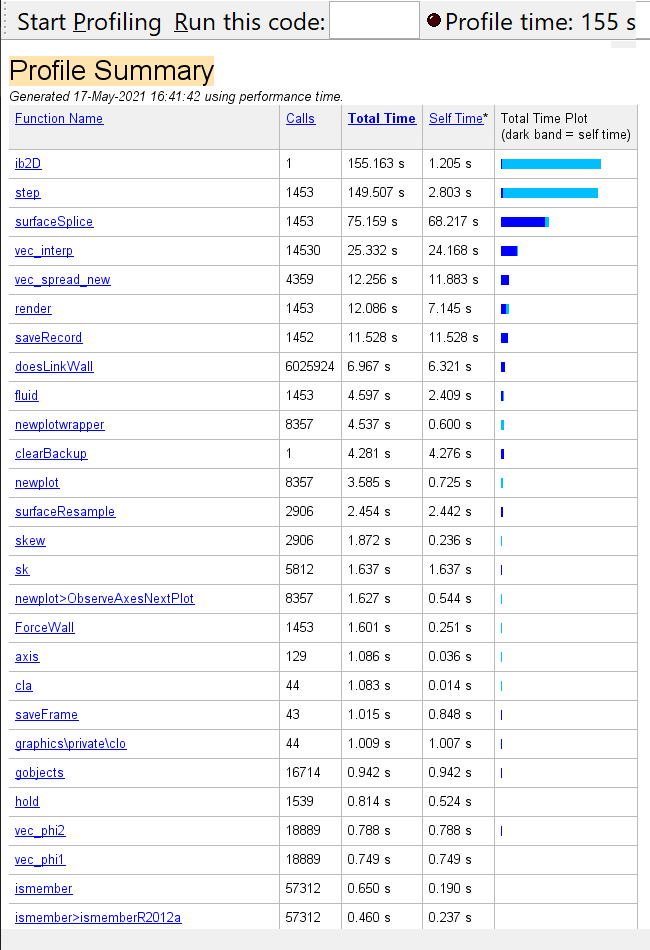
\includegraphics[width=4cm,trim={0mm 0mm 0mm 0mm},clip]{figs/time_profiling/summary.png}
        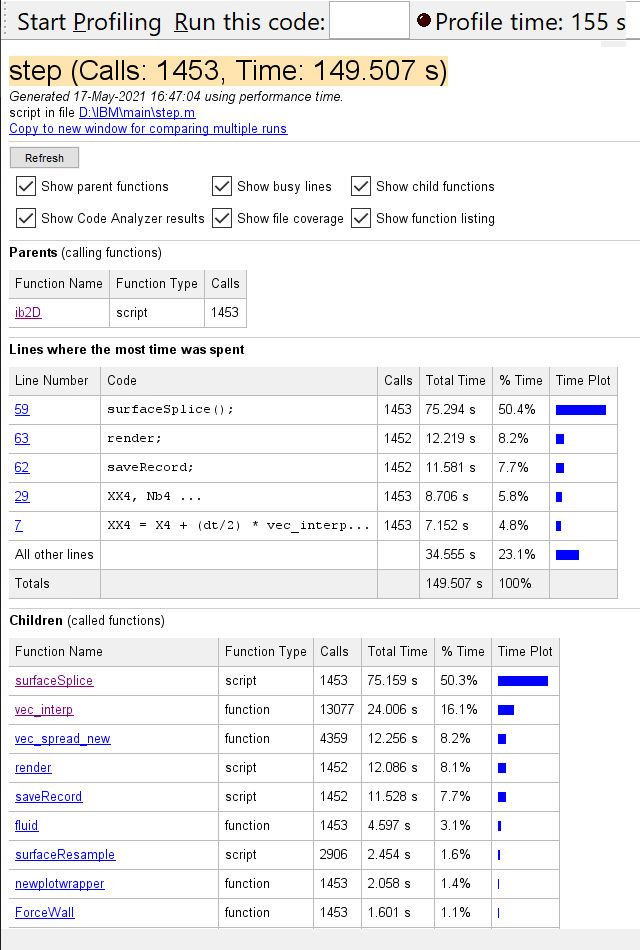
\includegraphics[width=4cm,trim={0mm 0mm 0mm 0mm},clip]{figs/time_profiling/step.png}
    \end{center}
    \begin{center}
        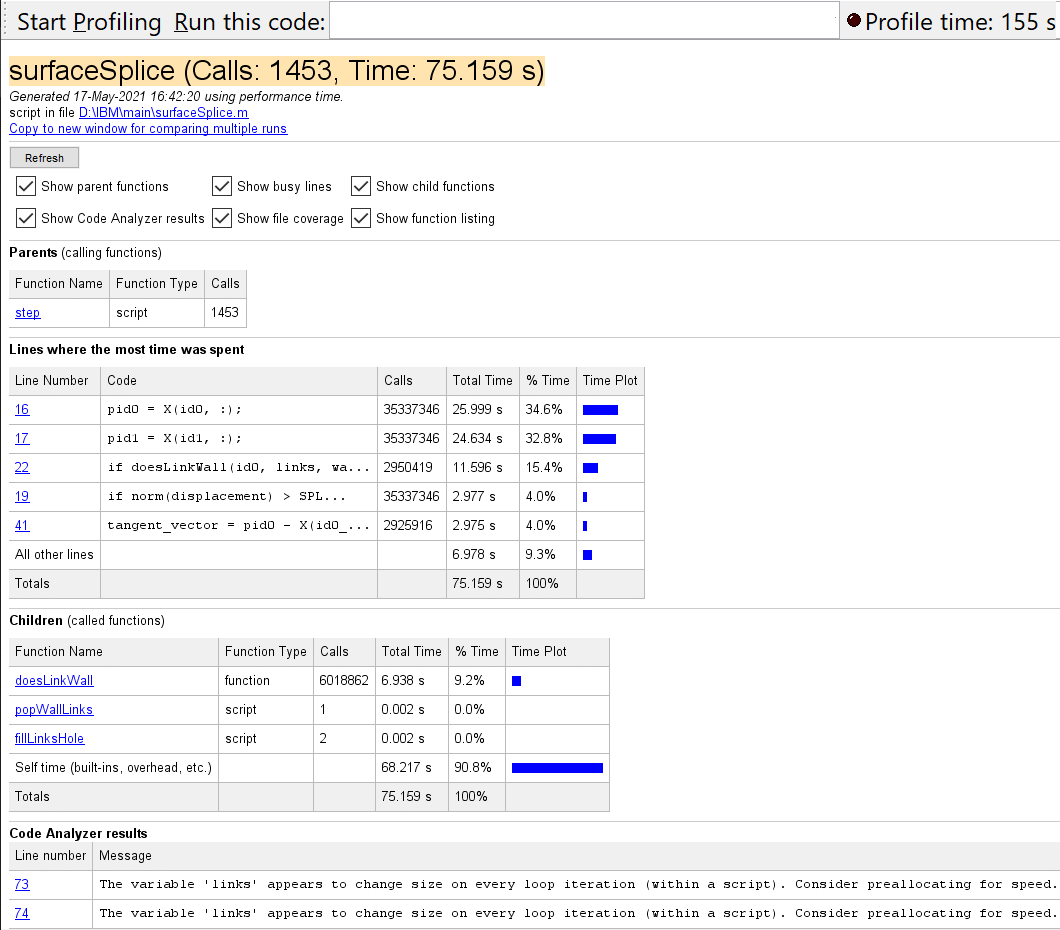
\includegraphics[width=6cm,trim={0mm 0mm 0mm 0mm},clip]{figs/time_profiling/surfaceSplice.png}
        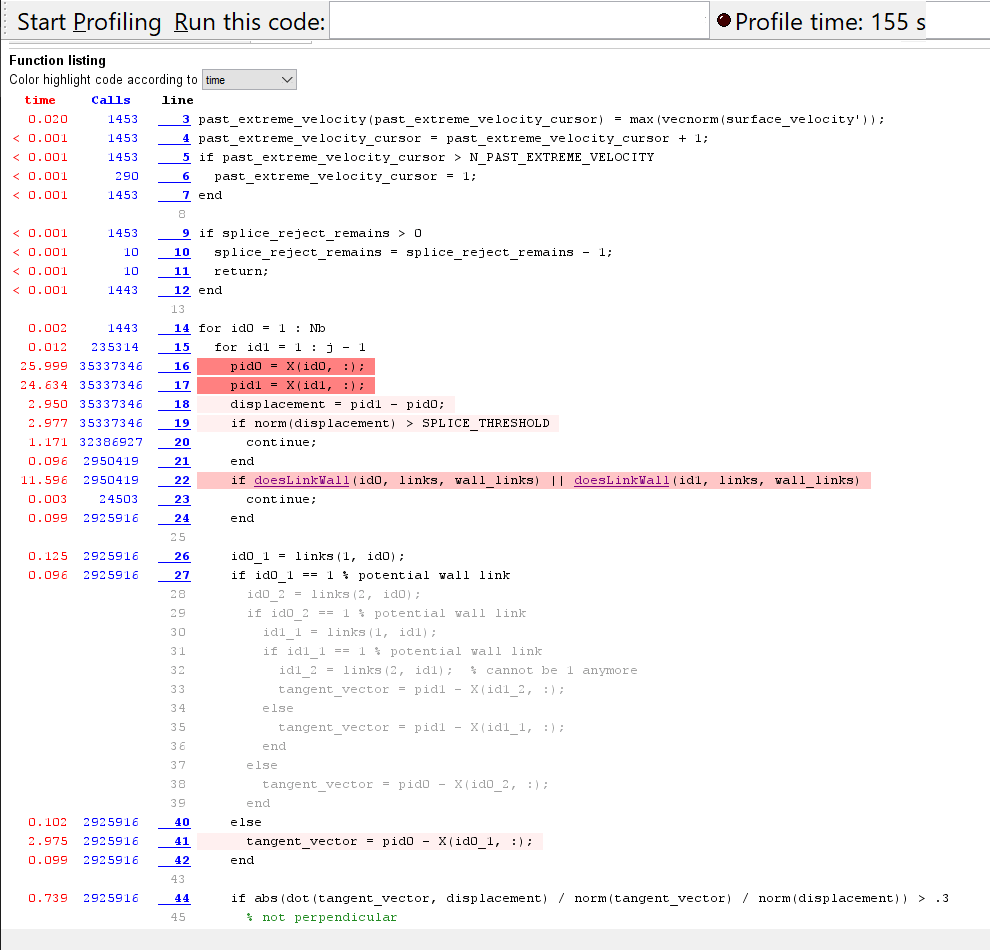
\includegraphics[width=6cm,trim={0mm 0mm 0mm 0mm},clip]{figs/time_profiling/code.png}
    \end{center}
    variable density
    demo dt instability (resample or surface tension)
    surfacesplice is expensive. vec interp in Kim et al is expensive. 

\section{Conclusions\label{sec:conclusion}}


 
\section*{Acknowledgements} 
We thank Otto Mierka and Stefan Turek for providing 10:10 benchmark data. 
\bibliographystyle{jfm}
\bibliography{mybibfile}
% \begin{thebibliography}{99}


% \bibitem[Sanaei {\it et al.}(2016)]{Sanaei2016}
% {\sc Sanaei, P., Richardson, G.W., Witelski, T., Cummings, L.J.,}
% Flow and Fouling in a Pleated Membrane Filter.
% {\it J. Fluid Mechanics.} {\bf 795}, 36-59 (2016).

% \bibitem[Sanaei {\it et al.}(2017)]{Sanaei2017}
% {\sc Sanaei, P., Cummings, L.J.,}
% Flow and fouling in membrane filters: Effects of membrane morphology.
% {\it published at J. Fluid Mechanics.} (2017)

% %\bibitem[Sanaei {\it et al.}(2017)]{Sanaei2017cake}
% %{\sc Sanaei, P., Cummings, L.J.,}
% %Optimum Permeability Profile and Fouling in Membrane Filters.
% %{\it Preprint.}



% \end{thebibliography}





\end{document}             % End of document.
